\documentclass{beamer}
%pkgs
\usepackage[utf8]{inputenc}
\usepackage[T1]{fontenc}
\usepackage{amsmath}
\usepackage{graphicx}
\usepackage{booktabs}
\usepackage{changepage}
\usepackage{listings}
\usepackage{xcolor}
\usepackage{textcomp}
\usepackage{pdfpages}

\usepackage{natbib}


\definecolor{codebg}{HTML}{EEEEEE}
\definecolor{codeframe}{HTML}{CCCCCC}
%themes
\mode<presentation>
{ \usetheme{boxes} }
\setbeamertemplate{navigation symbols}{}

%listings settings
\lstset{language=R}
\lstset{backgroundcolor=\color{codebg}}
\lstset{frame=single}
\lstset{framesep=10pt}
\lstset{rulecolor=\color{codeframe}}
\lstset{upquote=true}
\lstset{basicstyle=\ttfamily\footnotesize}
\lstset{showstringspaces=false}

\lstset{columns=flexible}
\lstset{keepspaces=true}

\makeatletter
\def\lst@outputspace{{\ifx\lst@bkgcolor\empty\color{white}\else\lst@bkgcolor\fi\lst@visiblespace}}
\makeatother

\lstdefinestyle{fullFunc} {language=R, showstringspaces=false, upquote=true, basicstyle=\ttfamily\tiny}

\newcommand\Wider[2][3em]{%
\makebox[\linewidth][c]{%
  \begin{minipage}{\dimexpr\textwidth+#1\relax}
  \raggedright#2
  \end{minipage}%
  }%
}

\title{Refactoring the {\bfseries xtable} package}
\author[Daniel Geals]{Daniel Geals\\{\small Supervised by: Paul Murrell and David Scott}}
\date{November 18, 2014}

\AtBeginSection[]
{
\begin{frame}<beamer> 
\frametitle{Outline} % make a frame titled "Outline"
\tableofcontents[currentsection]  % show TOC and highlight current section
\end{frame}
}




\setbeamertemplate{footline}[frame number]
\begin{document}


\begin{frame}
\titlepage
\end{frame}

\section{What is {\bfseries xtable}}

\begin{frame}[fragile]
\frametitle{{\bfseries xtable} example: R code}
		\begin{lstlisting}[language=R]
		library(xtable)
		
		#make some random data
		words = rep(c("low", "medium", "high") ,3)
		x = data.frame(var1 = rnorm(n = 9, mean = 10, sd = 2),
					   	           var2 = rnorm(n = 9, mean = 5, sd = 15),
			       		       var3 = runif(n = 9, min = -4, max = 4),
			       		       var4 = rnorm(n = 9, mean = 0, sd = 100),
			       		       factor = factor(sample(words)))
		
		#create LaTeX table with xtable
		tbl = xtable(x, digits = 2, 
		  			          caption = "data frame of random data 
		  			                     with booktabs option")
		align(tbl) = c("|lr|r|r|r|l|")
		print(tbl, booktabs = TRUE)
		\end{lstlisting}
\end{frame}

\begin{frame}[fragile]
\frametitle{{\bfseries xtable} example: LaTeX output}
		\begin{lstlisting}
		\begin{table}[ht]
		\centering
		\begin{tabular}{|lr|r|r|r|l|}
		  \toprule
		 & var1 & var2 & var3 & var4 & factor \\ 
		  \midrule
		  1 & 14.13 & -7.14 & -2.11 & 112.00 & low \\ 
		  2 & 10.78 & -10.76 & -2.85 & 97.42 & low \\ 
		  3 & 8.43 & -21.03 & 2.60 & 38.07 & medium \\ 
		  4 & 8.71 & -12.83 & -2.73 & 145.81 & low \\ 
		  5 & 8.46 & 39.89 & -3.13 & 36.43 & medium \\  
		  8 & 10.15 & 7.12 & 3.53 & -213.87 & high \\ 
		  9 & 12.09 & -22.52 & 2.21 & 94.50 & medium \\ 
		   \bottomrule
		\end{tabular}
		\caption{data frame of random data with booktabs option} 
		\end{table}
		\end{lstlisting}
\end{frame}

\begin{frame}
  \frametitle{{\bfseries xtable} example}
  
  		\begin{table}[ht]
  		\centering
  		\begin{tabular}{|lr|r|r|r|l|}
  		  \toprule
  		 & var1 & var2 & var3 & var4 & factor \\ 
  		  \midrule
  		  1 & 14.13 & -7.14 & -2.11 & 112.00 & low \\ 
  		  2 & 10.78 & -10.76 & -2.85 & 97.42 & low \\ 
  		  3 & 8.43 & -21.03 & 2.60 & 38.07 & medium \\ 
  		  4 & 8.71 & -12.83 & -2.73 & 145.81 & low \\ 
  		  5 & 8.46 & 39.89 & -3.13 & 36.43 & medium \\  
  		  8 & 10.15 & 7.12 & 3.53 & -213.87 & high \\ 
  		  9 & 12.09 & -22.52 & 2.21 & 94.50 & medium \\ 
  		   \bottomrule
  		\end{tabular}
  		\caption{data frame of random data with booktabs option} 
  		\end{table}
  
\end{frame}

\begin{frame}
  \frametitle{About {\bfseries xtable}}
  \begin{itemize}
    \item {\bfseries xtable} is an R extension package that provides functionality for outputting \LaTeX \ and HTML code that when processed creates a table\\
    \item we can create a table with few lines of code but the package has many optional arguments for customisation\\
    \item {\bfseries xtable} is geared toward \LaTeX \ table production with many \LaTeX \ specific arguments but few for HTML\\
    \item {\bfseries xtable} is useful in the literate programming and reproducible document arena\\
    \item {\bfseries xtable} mitigates risks inherent in creating \LaTeX \ and HTML tables 'by hand'
  \end{itemize}
\end{frame}

\section{Issues with {\bfseries xtable}}

\begin{frame}[fragile]
  \frametitle{Existing implementation}
  \vspace{-4mm}
  \Wider[4em]{
  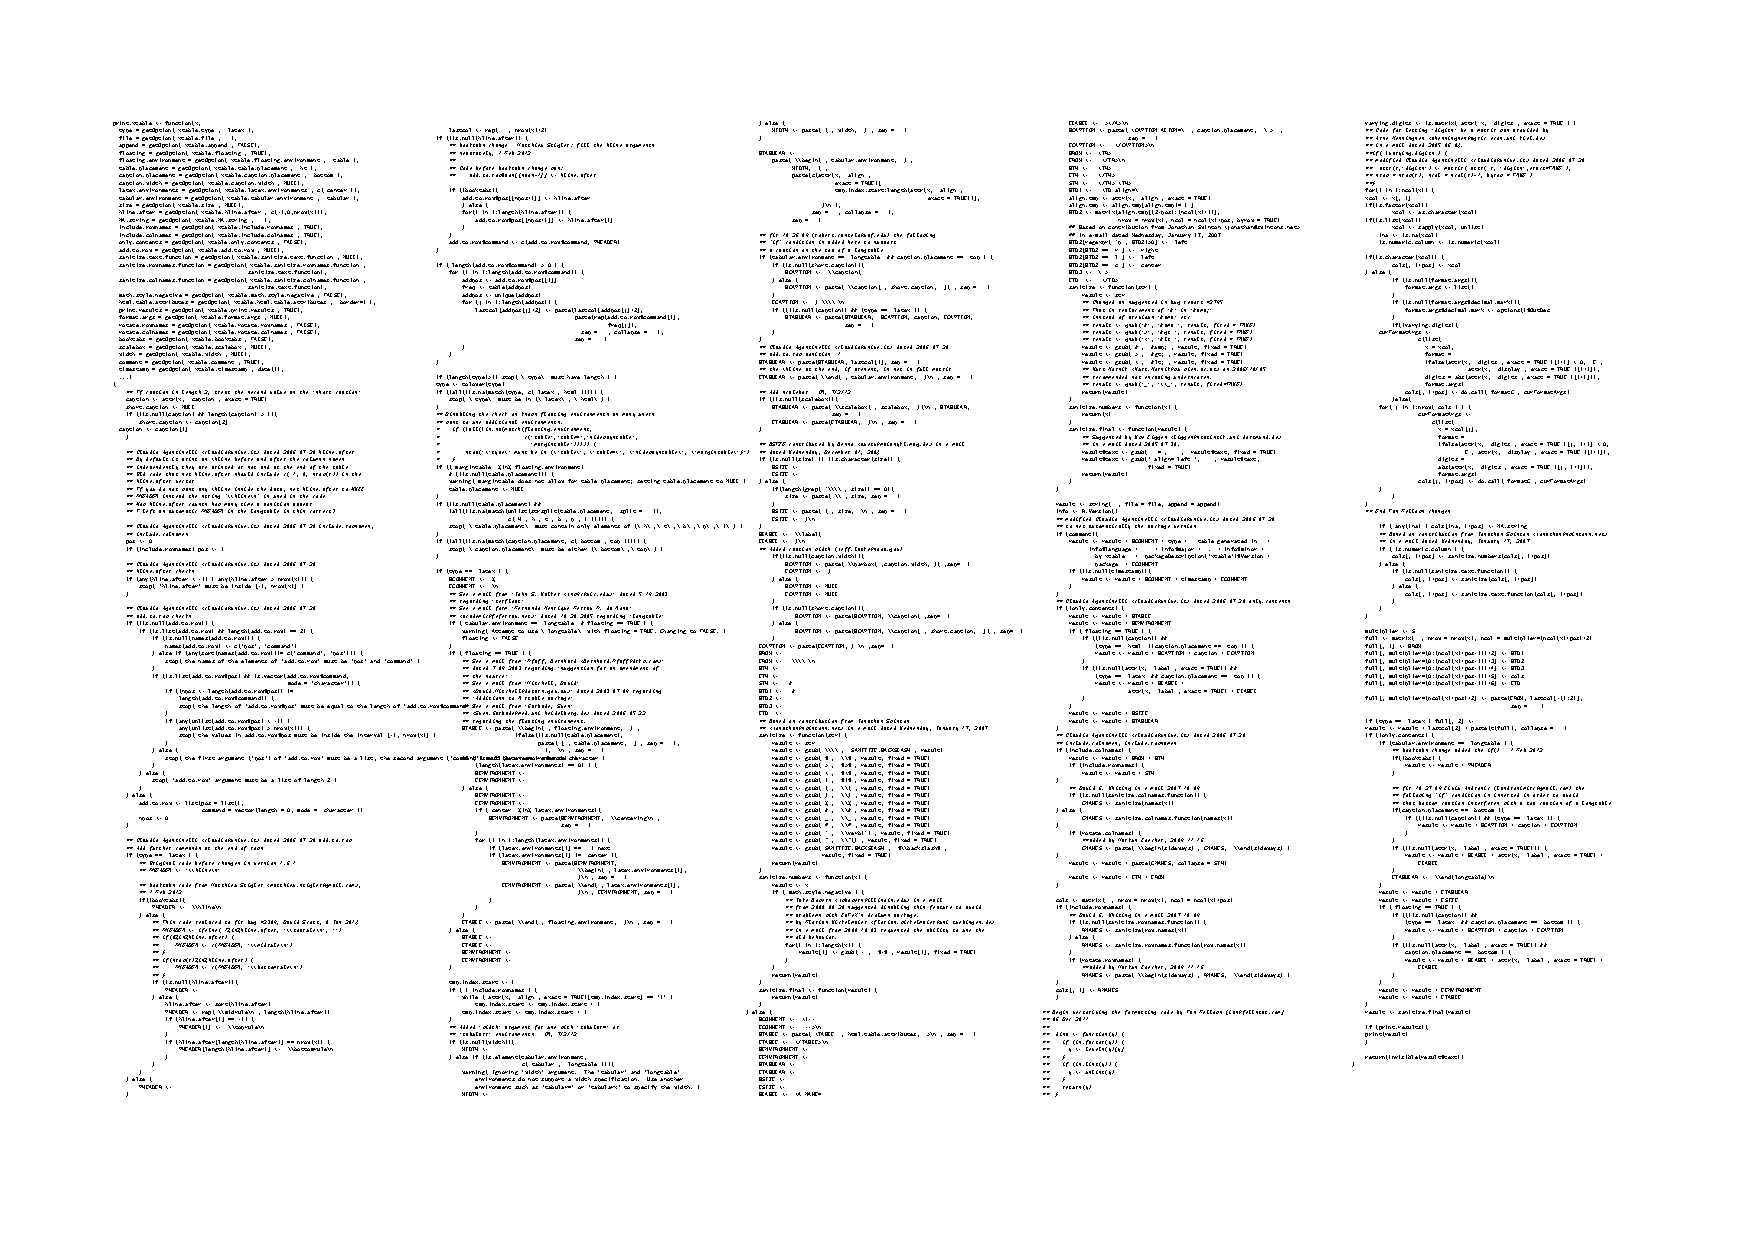
\includegraphics[width=13cm]{code.pdf}}
\end{frame}


\begin{frame}
\frametitle{Issues with existing implementation}

\begin{itemize}
  \item \texttt{print.xtable}
  \item mixture of \LaTeX\ environments and HTML
  \item large number of function arguments\\
  \item 650 line function\\
  \item too many different operations taking place in one function\\
  \item package is difficult to maintain\\
  \item hard to add additional functionality\\
  \item not following proper programming practice\\
\end{itemize}

\end{frame}

\section{Refactoring}

\begin{frame}
  \frametitle{Refactoring definition}
  \begin{exampleblock}{}
    {\large ``Refactoring is the process of changing a software system in such a way that it does not alter the external behaviour of the code yet improves its internal structure. It is a disciplined way to clean up code that minimises chances of introducing bugs.''}
    \vskip5mm
    \hspace*\fill{\small--- Martin Fowler, Refactoring}
  \end{exampleblock}
\end{frame}
%http://martinfowler.com/bliki/DefinitionOfRefactoring.html


\begin{frame}
\frametitle{Creating new functions}
  \vspace{-5mm}
  \begin{figure}
    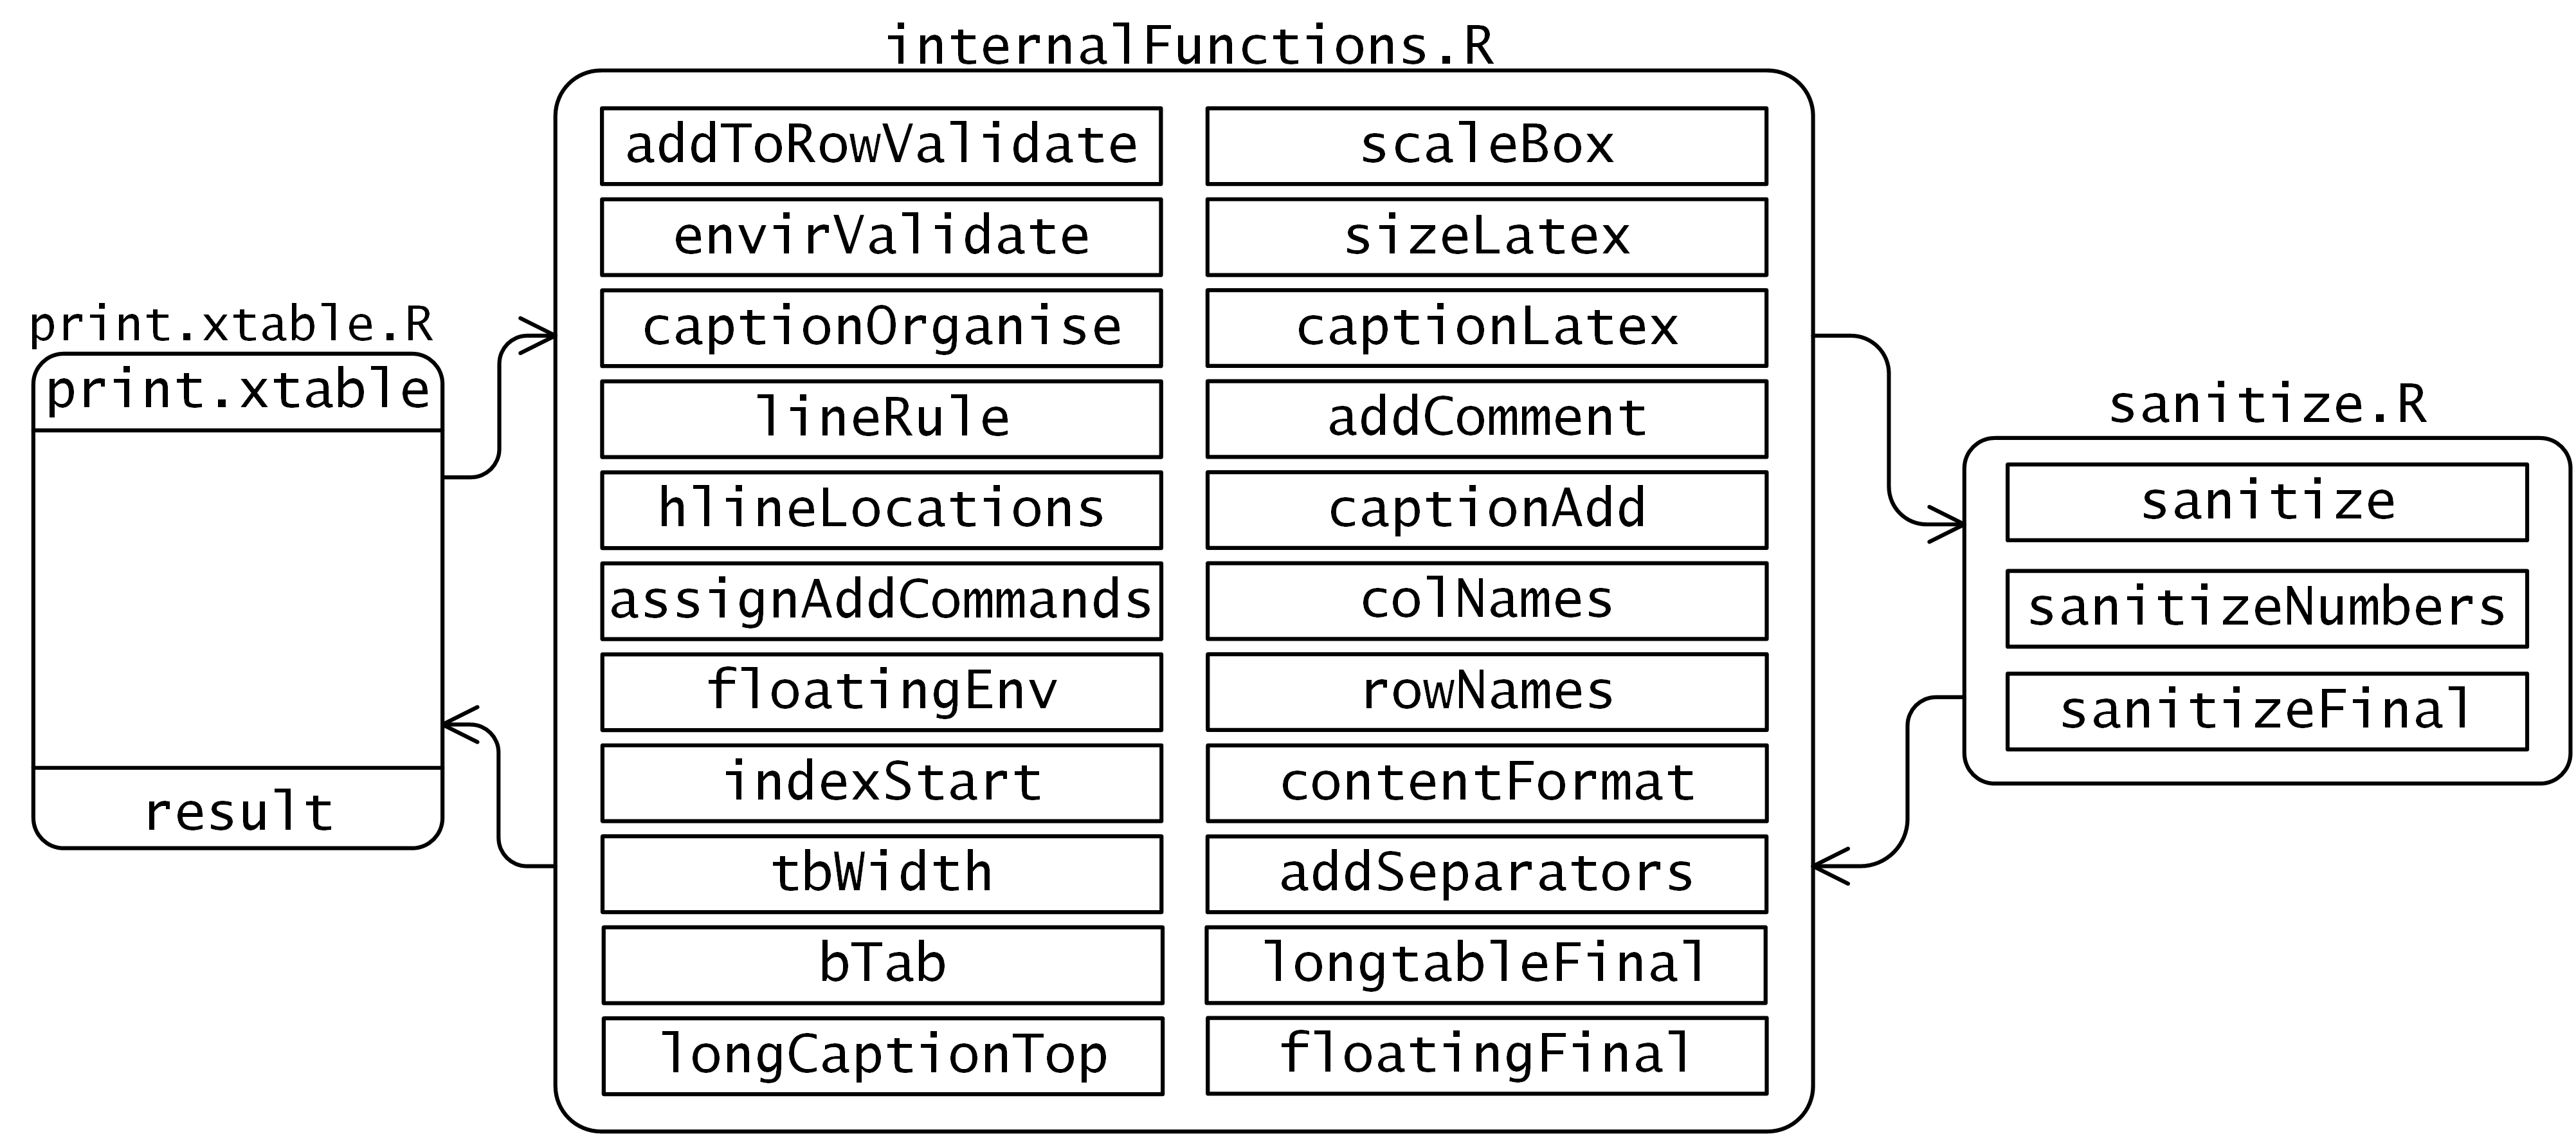
\includegraphics[width=11cm]{stage1.png}
  \end{figure}
\end{frame}

\begin{frame}
  \frametitle{Restructuring}
  \vspace{-5mm}
  \begin{figure}
    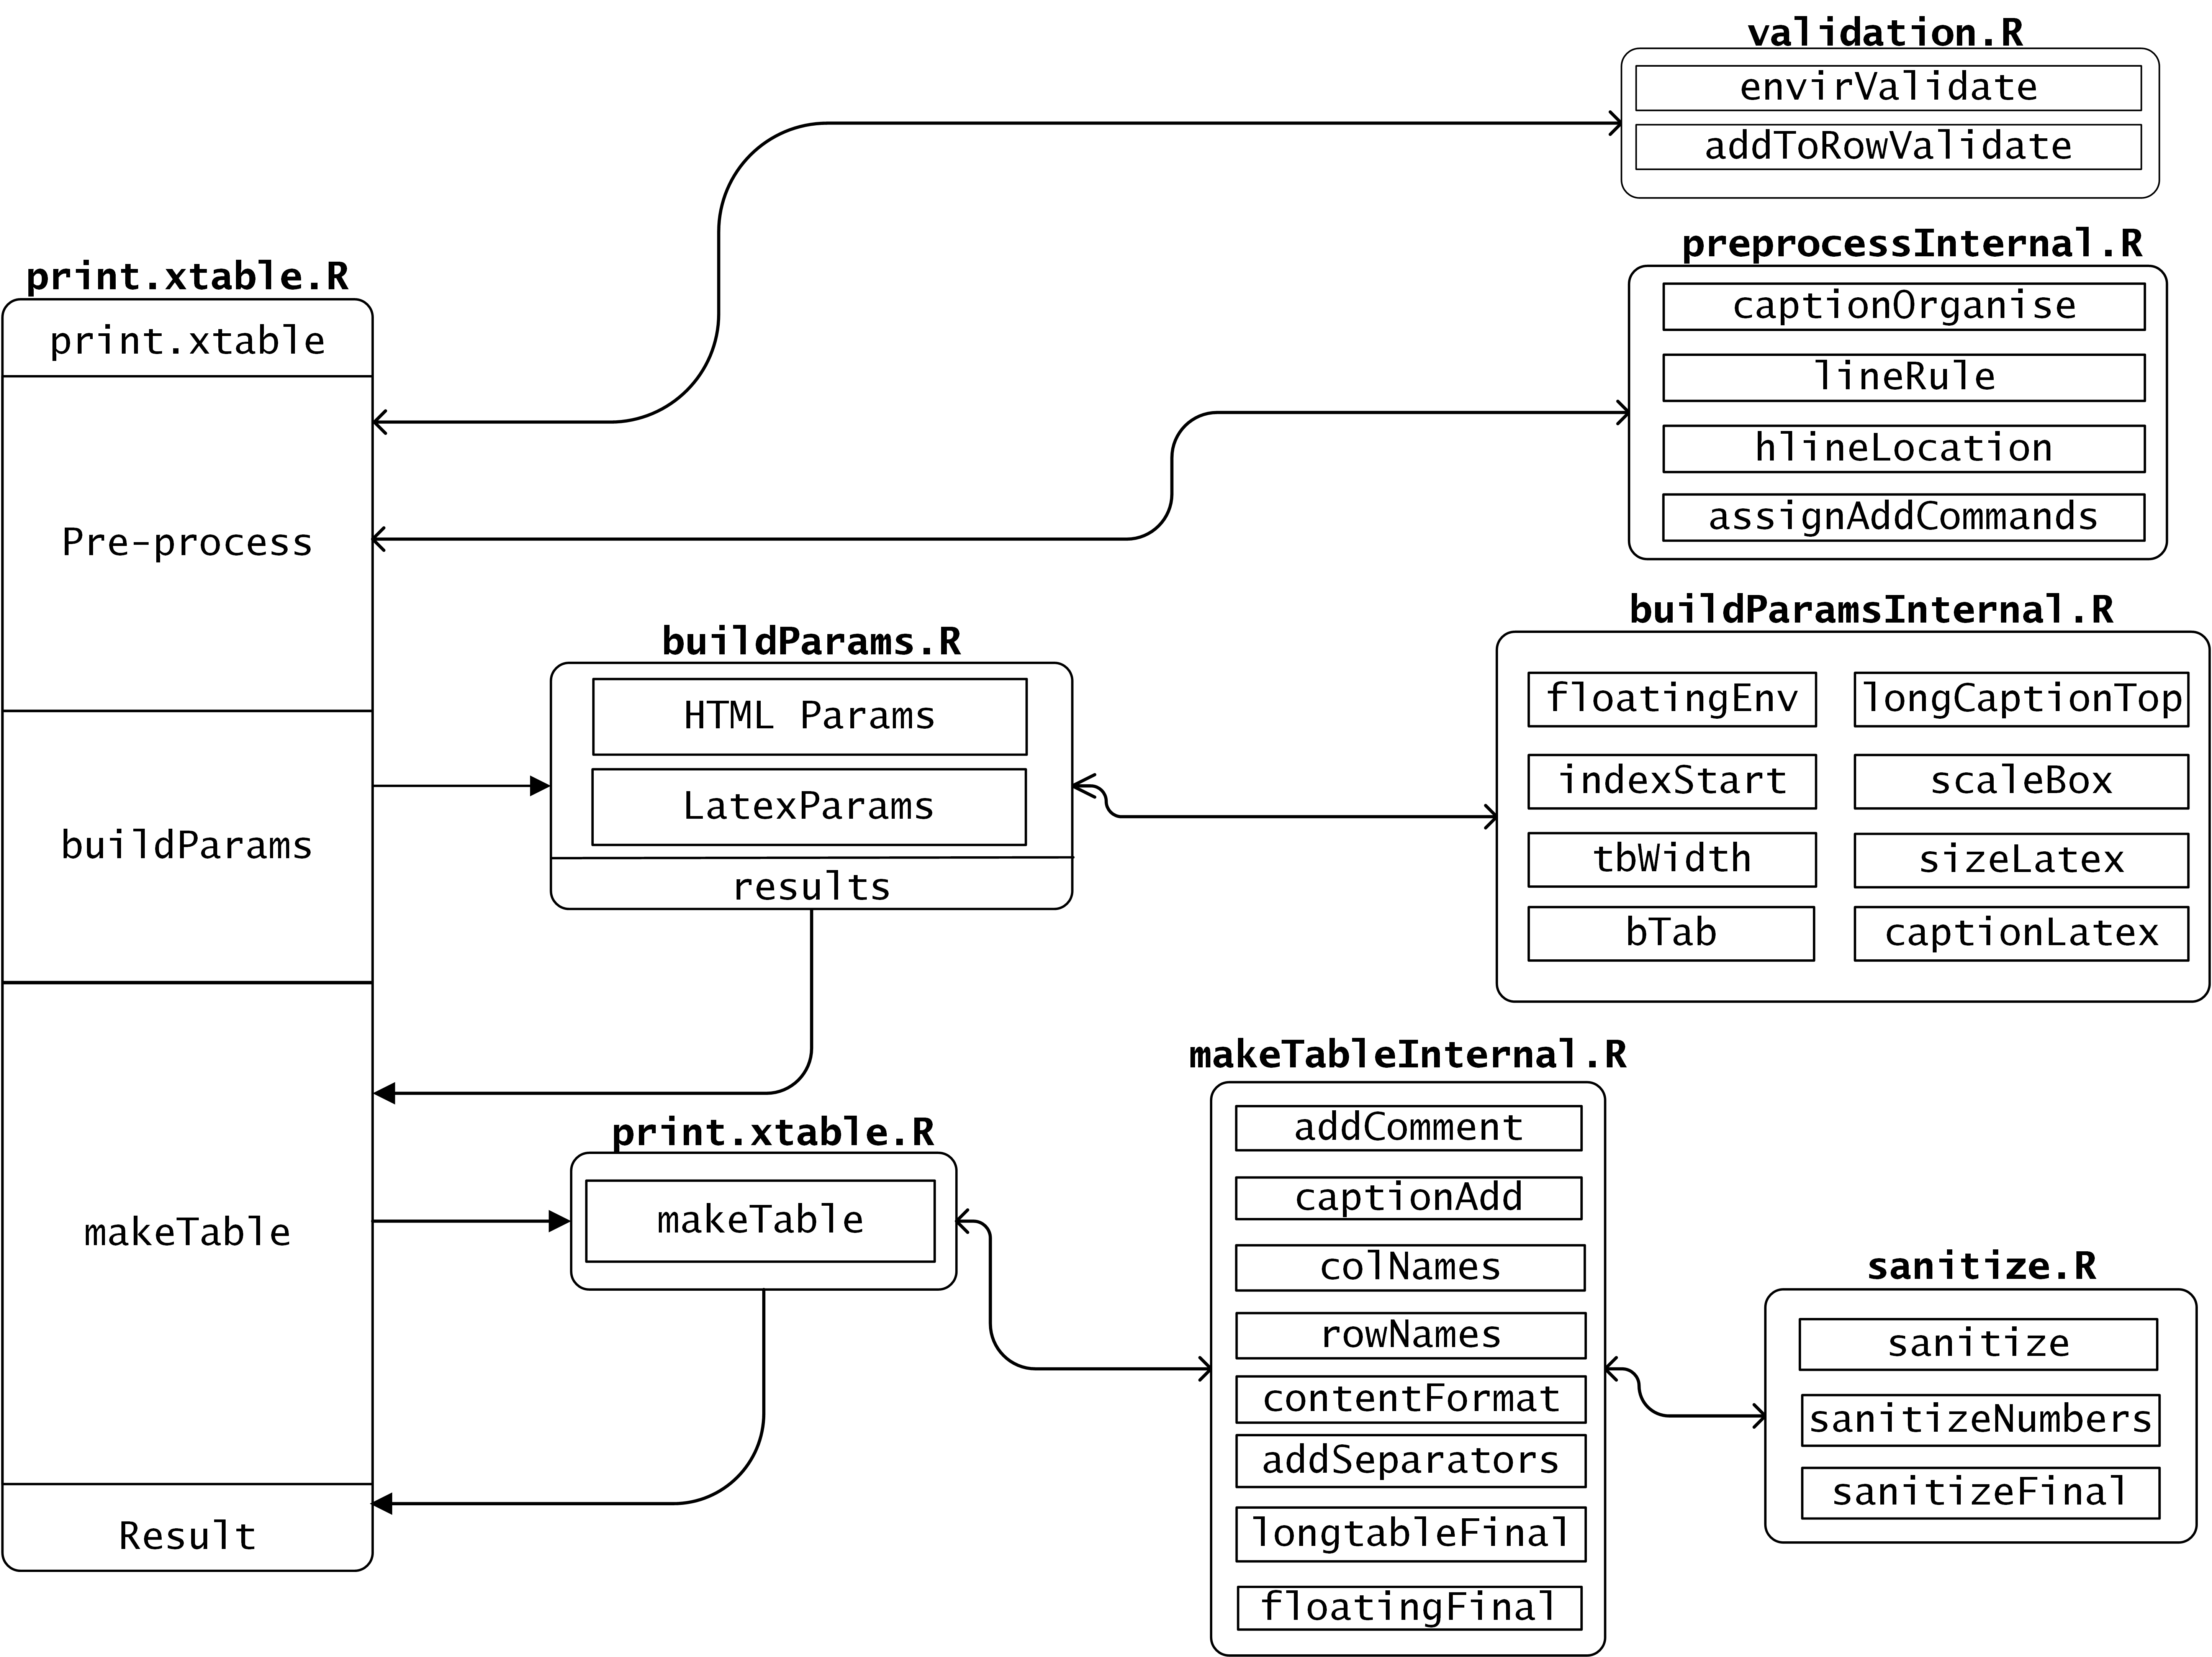
\includegraphics[width=11cm]{refactored.png}
  \end{figure}
\end{frame}

\begin{frame}
	\frametitle{Summary of changes made}
	 \begin{itemize}
		 \item extract the lower level programmatic detail into internal functions\\
		 \item give reasonably descriptive names to new functions\\
		 \item minimise amount of activity in new functions\\
		 \item remove some of the old comments, especially commented out code\\
		 \item attempt to restructure the code with larger functions that call the newly created internal functions\\
	 \end{itemize}
\end{frame}

\section{Testing Procedures}

\begin{frame}
  \frametitle{Why we need testing}
  
  \begin{itemize}
    \item package must take inputs and return outputs that are exactly the same as the existing version (keep external behaviour)\\
    \item large number of arguments that need to be tested as working\\
    \item combinations of these arguments also need to be tested as working\\
    \item invalid combinations of arguments need to be rejected with appropriate error messages\\
    \item having appropriate tests can form the basis of a development cycle\\
  \end{itemize}
\end{frame}

\begin{frame}
  \frametitle{Testing procedures}
   Confirm changes have not broken the package
  \begin{itemize}
    \item use the provided gallery to test if modified functions create identical content
    \item use a diff utility to compare line by line between the old and new gallery
   \end{itemize} 
   Confirm invalid input is returning appropriate errors
    \begin{itemize}
      \item create test suite using {\bfseries testthat} package
      \item test that invalid inputs are being stopped by the validation functions
    \end{itemize}
  Ensure tests return informative output and are convenient to run
\end{frame}

\begin{frame}[fragile]
	\frametitle{Testing example}
	\begin{lstlisting}[language=R]

		test_that("Long table warning works", {
		  data(tli)
		  tli.table <- xtable(tli[1:10,])
		  #check floating and longtable combination gives warning
		  expect_that(print(tli.table, tabular.environment = "longtable", 
	                    floating = TRUE), gives_warning())
		})
	\end{lstlisting}
\end{frame}

\section{Conclusion}

\begin{frame}[fragile]
  \frametitle{Existing implementation}
  \vspace{-4mm}
  \Wider[4em]{
  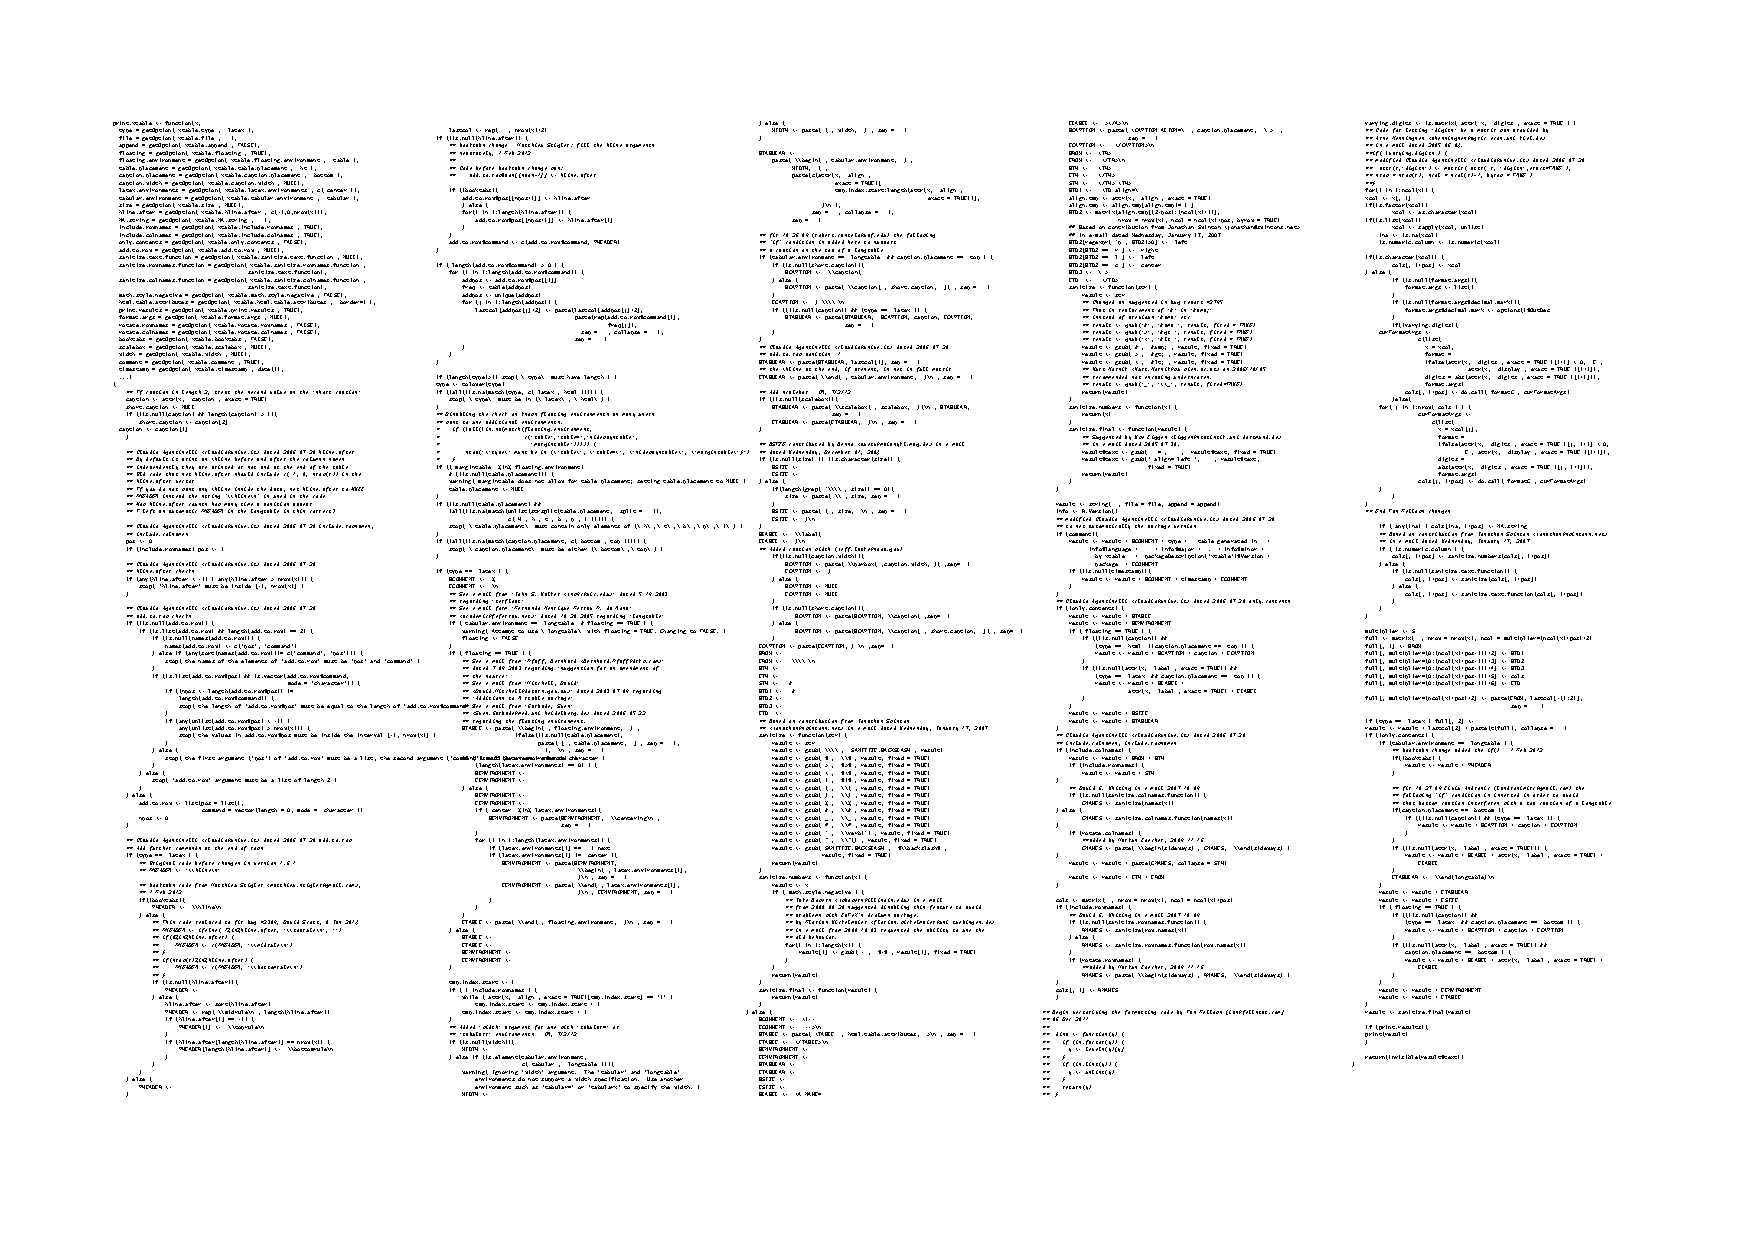
\includegraphics[width=13cm]{code.pdf}}
\end{frame}


\begin{frame}[fragile]
  \frametitle{Refactored version}
  \vspace{-4mm}
  \Wider[4em]{
  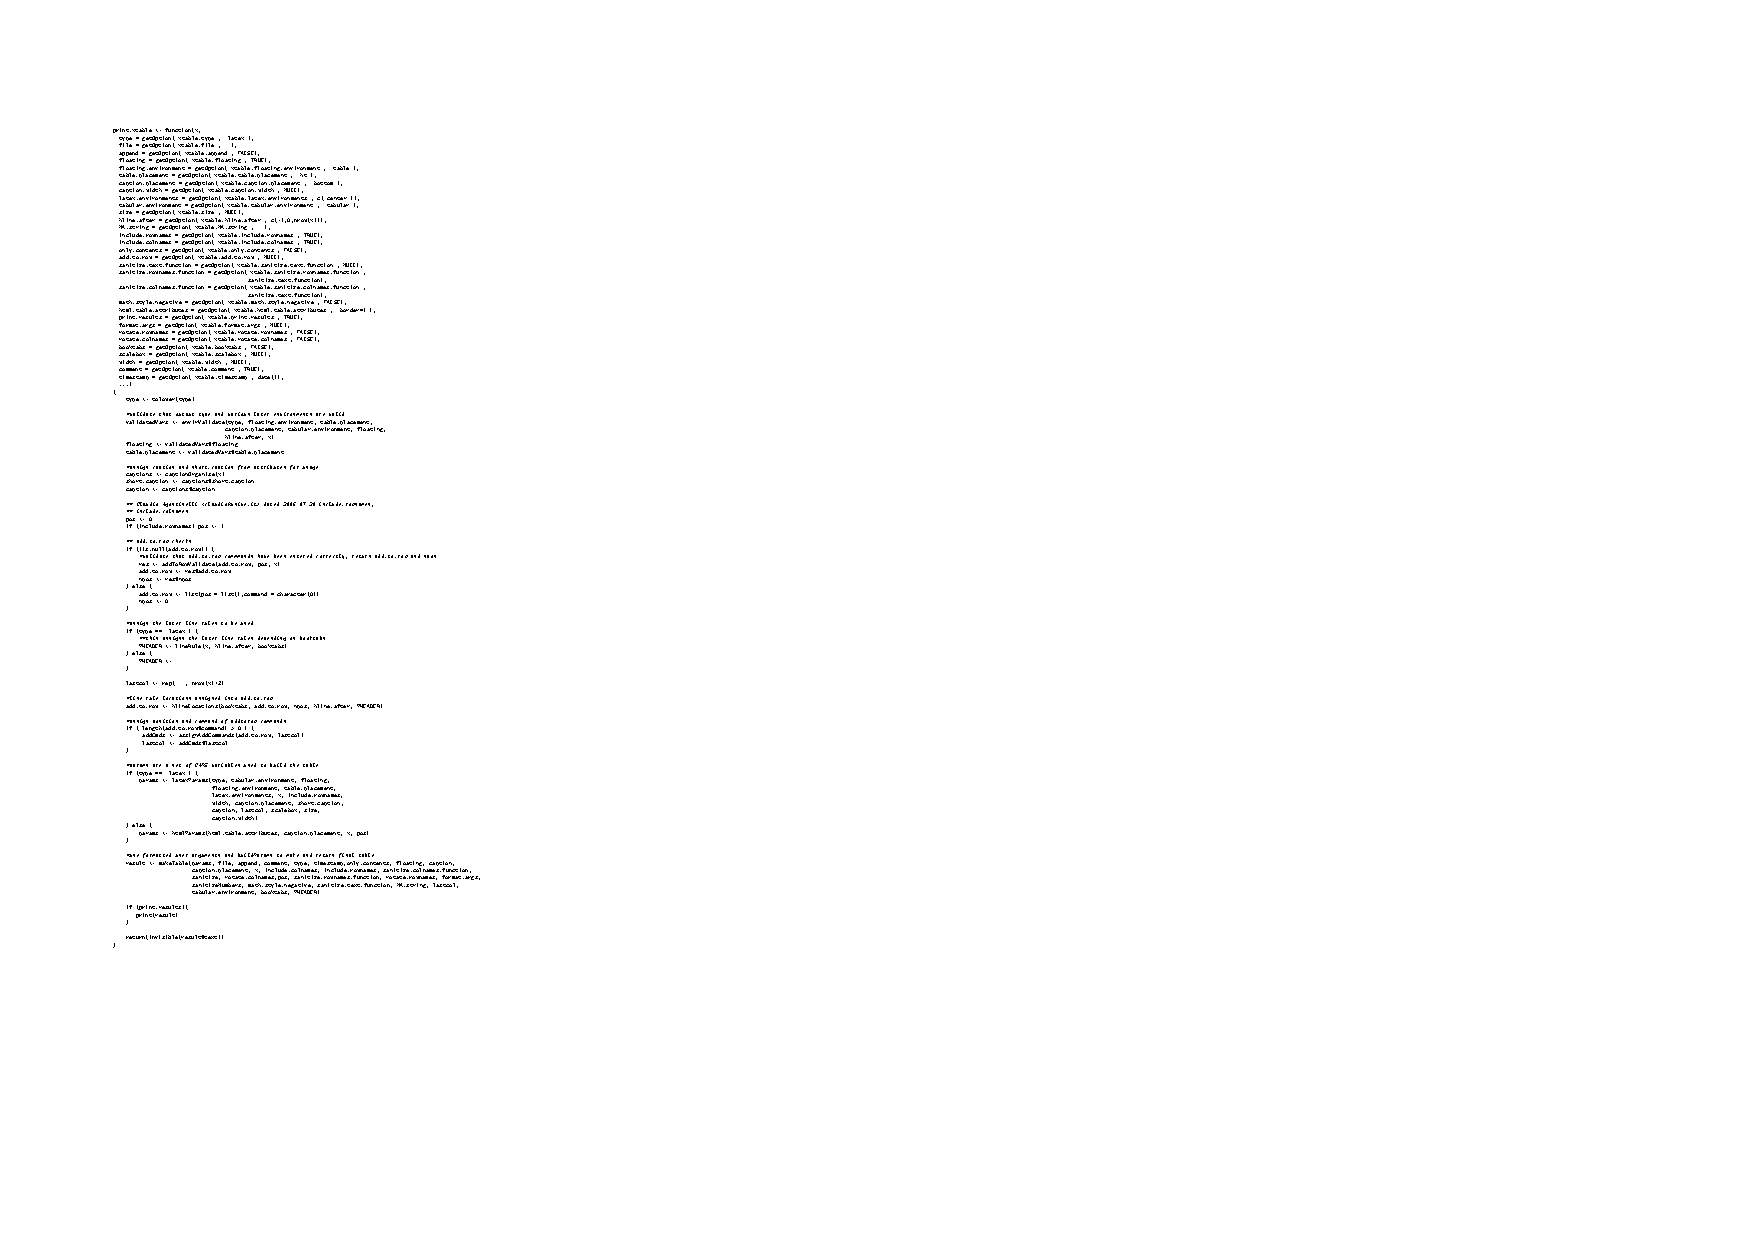
\includegraphics[width=13cm]{finalcode.pdf}}
\end{frame}

\begin{frame}
	\frametitle{Conclusions}
	\begin{itemize}
	\item function of issue has been refactored
	\item backwards compatibility
	\item future work
	\end{itemize}
	
\end{frame}

\begin{frame}
\frametitle{References}
	\nocite{*}
	\bibliographystyle{apalike}
	\bibliography{references}
\end{frame}

\end{document}
